% CAS (Heimdall) -- system functional description: outlet system (hydraulic outlet dampers)
% Structure: Cooling, Software Engineering for Real-Time Systems (2020), sec. 14.3 [COO]
\documentclass[11pt,a4paper]{article}
% casfd.sty defines \tag with \newcommand after loading amsmath, which already has \tag.
\usepackage{amsmath}
\usepackage{casfd}
\usepackage{adjustbox}

\casfdheader{Outlet system}{CAS-FD-30}{A}

\newcommand{\prop}{\textsuperscript{\dag}}  % proposed tag, not on the P&ID set
\newcommand{\TBD}{\textcolor{red}{TBD}}

\begin{document}
\maketitle

\begin{abstract}
\noindent The bottom outlet of the CAS closed pen has four dampers. Each damper is moved by a
hydraulic cylinder. A Servi hydraulic power unit (HPU) with a four-section HAWE PSL valve bank
drives the cylinders. The CAS PLC sets all four dampers to a common opening per operating mode. It
finds the position of each cylinder by counting pulses from an oil-flow meter, and detects end
positions by a rise in line pressure. This document describes the equipment, the control principle,
the sequences, interlocks and faults, and lists what is still open. It describes the PLC function
as implemented in \var{FB.Outlet.OutletControl}; it does not redesign it.
\end{abstract}

\setcounter{tocdepth}{1}
\tableofcontents
\clearpage

% =====================================================================================================
\section{Introduction}
\label{sec:intro}

\subsection{Purpose}
This document is the system functional description of the outlet system of the CAS (Heimdall)
closed fish pen. It is written for engineers, operators, the project team and the suppliers
(Østerbø Solutions, Servi). After reading it, the reader should know:
\begin{itemize}[nosep]
  \item which instruments and actuators the outlet has, and where their signals go;
  \item how the PLC finds the damper position and moves the dampers;
  \item what happens on start-up, stop, faults, emergency stop and power loss;
  \item which questions are still open.
\end{itemize}
The structure follows Cooling's system functional specification [COO, §14.3]: block diagram
description (§14.3.2, Section~\ref{sec:block}), functional diagram description (§14.3.3,
Section~\ref{sec:func}), and the requirements specification, functional (§14.3.4a,
Section~\ref{sec:freq}) and non-functional (§14.3.4b, Section~\ref{sec:nfreq}).

\subsection{Scope}
In scope: the four outlet dampers, the four cylinders, the HPU and valve cabinet (Servi order
S6377070), junction box JB1 (Servi drawing 18068) with its local operation panel, the signals to the
CAS remote I/O (CommonRIO), the PLC function block \var{FB.Outlet.OutletControl}, and the operator
functions on the HMI.

Out of scope: the dead fish pump (DC-81) and sludge pump (SS-91) at the outlet, which Barge Control
controls; the level control LIC01, which uses the operating mode set here but is described in the
inlet FD; the mechanical design of the dampers (Østerbø).

\subsection{Sources}
\begin{small}
\begin{tabularx}{\textwidth}{@{}lL@{}}
\toprule
ID & Document \\
\midrule
{[COO]}  & J. Cooling, \emph{Software Engineering for Real-Time Systems}, 2020, §14.3 System functional specifications \\
{[FD]}   & P-15169-CAS-FD-01 Funksjonsbeskrivelse CAS, rev.~B, §3.2.3 Utløpsspjeld (Norwegian) \\
{[AL]}   & P-15169-CAS-FD-02 Alarmliste CAS Heimdall, rev.~A \\
{[A1]}   & Servi 2939238 rev.~A1, Hydraulikk skjema, spjeld til utløp HY, art.~810936, 18.06.2026 (current) \\
{[T1]}   & Servi 2799175 rev.~T1, HPU for spjeld til utløp, hydraulic schematic for the offer, 09.04.2025 (superseded) \\
{[JB]}   & Servi 18068 rev.~A3, El interface for spjeldventiler (JB1 and operation panel ST-16183), 16.10.2026 \\
{[QNA]}  & QnA Servi hydraulikksystem CAS, meeting notes 18.02.2026 \\
{[MAIL]} & E-mail thread ``S6377070 / 25031 Automatisk stenging'', 28.09.--19.10.2026 (Servi, Østerbø, ScaleAQ) \\
{[QG]}   & HySense QG100 gear flow meter, data sheet and TED \\
{[TDS]}  & Hoyer HMA3 90L-4 1.5\,kW motor data sheet; Marzocchi GHP gear pump data sheet \\
{[HMD]}  & Hemomatik HMDHI level / temperature switch data sheet \\
{[PID]}  & CAS P\&ID and loop diagrams: CAS-PID-500 (outlet), LD-806 (loop), I/O list, open points \\
{[DB]}   & CAS design basis (System Modelling) and the outlet simulator CasOutletSim (\texttt{design\_basis.toml}) \\
{[PLC]}  & Heimdall PLC export: \var{FB.Outlet.OutletControl}, DUT \var{System.Outlet}, \var{FB.RIO.CommonRIO}, PFC200\_Sim \var{ConfigValues} \\
{[AKS]}  & Aksjonsliste CAS styresystem (items 23, 41, 42, 81, 82, 91); CAS PLS aksjonsliste (item 6) \\
\bottomrule
\end{tabularx}
\end{small}

\subsection{Abbreviations and conventions}
\begin{small}
\begin{tabularx}{\textwidth}{@{}lL@{\hspace{6mm}}lL@{}}
\toprule
HPU & Hydraulic power unit (tank, pump, motor, valves) & PSL & HAWE proportional directional valve, load sensing \\
JB1 & Servi junction box 18068 at the HPU & DOL & Direct-on-line motor starter \\
CommonRIO & WAGO 750-362 remote I/O node in the CAS cabinet & DO / DI / AI & Digital out / digital in / analog in \\
Plus stroke & Rod out, oil into the A (piston) side & Minus stroke & Rod in, oil into the B (rod) side \\
O-35 \dots S-75 & Operating modes (O = operation, S = service; number = residence time in minutes) & FAT & Factory acceptance test \\
\bottomrule
\end{tabularx}
\end{small}

Tags follow the P\&ID set [PID] (ISA-5.1), printed as \itag{PT61}. Servi's own designations from
[A1] and [JB] are given in brackets, e.g.\ \itag{PT61} (1PT1). Tags marked \prop{} are proposed in
this document and are not yet on the P\&ID set. PLC names are printed as \var{Outlet.Cylinder[i].Status.Position};
cylinder index \var{i} = 0..3 is cylinder 1..4. Open issues are marked \open{n} and listed in
Section~\ref{sec:open}; decisions are marked \decided{n}. \TBD{} marks a number that is not known yet.

\subsection{Revision}
\begin{small}
\begin{tabularx}{\textwidth}{@{}llL@{}}
\toprule
Rev. & Date & Change \\
\midrule
A & 21.10.2026 & First issue. Written from [A1], [JB] rev.~A3, [FD] rev.~B and the PLC export, after the review of 21.10.2026.
  Records the power-loss decision \decided{1}. Supersedes [FD] rev.~B §3.2.3 on fail-to-close and XV65. \\
\bottomrule
\end{tabularx}
\end{small}

% =====================================================================================================
\section{Block diagram description}
\label{sec:block}

\subsection{Outlet arrangement}
The pen water leaves through a bottom centre outlet (\O\,5.5\,m [PID]). Four dampers sit in the
outlet; together they set the outlet conductance and thus, with the inlet pumps, the water exchange
and the over-height of the water in the pen. Each damper is moved by its own hydraulic cylinder
through a mechanical link (Østerbø design). In normal operation all four dampers have the same
opening, given by the operating mode [FD]. Each damper can also be moved on its own (manual mode),
for calibration and maintenance. Below the dampers, branches go to the dead fish and sludge
systems, which are not part of this description.

\subsection{Equipment}
\begin{small}
\begin{tabularx}{\textwidth}{@{}P{30mm}LP{26mm}@{}}
\toprule
Item & Description & Source \\
\midrule
Cylinders 1--4 & Double-acting, \O40/20$\times$300\,mm, Servi part 810872, type HRC-N-D-40/20x300-S (Servi A1 item 29).
  Piston area 12.57\,cm$^2$, annulus 9.42\,cm$^2$. Oil volume per full stroke: A side 0.377\,l, B side 0.283\,l. Acid-proof rod, double scrapers recommended. & [A1], [QNA] \\
Tank \itag{TL61} & 12\,l oil tank (Servi item 1), sight glass, breather filter. & [A1] \\
Pump \itag{PU61} & Fixed-displacement gear pump Marzocchi GHP1D4, 2.8\,cm$^3$/rev; 3.5\,l/min at 150\,bar (4.1\,l/min theoretical at 1450\,rpm). & [A1], [TDS] \\
Motor \itag{M61} (1M1) & Hoyer HMA3 90L-4, 1.5\,kW, 230/400\,V 50\,Hz, 3.4\,A, IE3, with PTC. DOL via KM1, motor protection breaker QM1. & [A1], [TDS], [JB] \\
Hand pump \itag{HP61}\prop & Hansa GL25 hand pump with check valve into the pressure line (Servi items 25--26). Manual override when the motor cannot run. & [A1] \\
Pressure relief & Main relief 150\,bar. Max.\ working pressure 150\,bar, design 170\,bar, test 190\,bar. & [A1] \\
Valve bank & HAWE PSL size 2, four sections (Servi item 21, 810855), load sensing, one section per cylinder.
  Two solenoids per section: \itag{XV61}..\itag{XV64} = 1YV1..1YV4, solenoids MB1--MB8 (24\,V DC, 680\,mA). Per section: port pressure limiters 100\,bar, over-centre (load-holding) valves 130\,bar on A and B. & [A1], [JB] \\
Flow meters \itag{FT61}..\itag{FT64} (1FT1..4) & HySense QG100, 0.05--5\,l/min, 0.191\,cm$^3$/pulse ($\approx$5200 pulses/l), square-wave output with direction detection (order no.\ 3146-02-35.0300). On the A line of each cylinder. & [A1], [QG] \\
Pressure transmitters \itag{PT61}, \itag{PT63}, \itag{PT65}, \itag{PT67} (1PT1..4) & PT5401, 0--250\,bar, 4--20\,mA, one per cylinder on the A line. The B-line transmitters \itag{PT62}..\itag{PT68} of [FD] are \emph{not} on [A1] \open{1}. & [A1], [JB] \\
Tank switch \itag{LSL61}/\itag{TSH61} (1SL1/1ST1) & Hemomatik HMDHI-OT1: low level (switch at 120\,mm) and over-temperature 70\,$^\circ$C, NC contacts in series, potential-free. & [A1], [HMD], [JB] \\
Filter switches \itag{PDS61}\prop, \itag{PDS62}\prop & Pressure filter (6\,bar bypass) and return filter (1.75\,bar bypass) clogging indicators 1PDS1/1PDS2, 24\,V, contacts in series (one signal). & [A1], [JB] \\
Gauge \itag{PI61} & Manometer \O63, 0--250\,bar, on Minimess test point; 9 further Minimess test points. & [A1] \\
JB1 & Servi junction box ST-18068/JB, IP66: terminals for all signals, main and backup 400\,V supply with contactors K1 (main) / K2 (backup, interlocked), motor contactor KM1, motor breaker QM1. & [JB] \\
Operation panel & Servi ST-16183 at the HPU: emergency stop \itag{ES61} (SE1), Stop (S2), Start with green running lamp (SH3). & [JB] \\
CommonRIO & WAGO 750-362 node in the CAS cabinet: 2$\times$750-638 counters, 750-455 analog inputs, 750-1405 DI, 750-1515 DO with interposing relays XK01--XK08. Modbus TCP to the PLC. & [PID], [PLC] \\
PLC & WAGO PFC200 CAS PLC, program \var{FB.Outlet.OutletControl}, called from \var{PRG.Main}. & [PLC] \\
HMI & CAS operator HMI (operating mode, manual / jog, calibration, alarms). & -- \\
\bottomrule
\end{tabularx}
\end{small}

Figure~\ref{fig:block} shows the physical and network structure. Figure~\ref{fig:hyd} shows the
hydraulics for one cylinder in simplified form, with the instruments as ISA bubbles; the other three
cylinders are identical.

\begin{figure}[htbp]
\centering
\begin{adjustbox}{max width=\linewidth}\begin{tikzpicture}[node distance=6mm and 8mm, font=\small]
  % pen outlet
  \node[proc, minimum width=22mm] (d1) at (0,9.2) {damper 1};
  \node[proc, minimum width=22mm, right=4mm of d1] (d2) {damper 2};
  \node[proc, minimum width=22mm, right=4mm of d2] (d3) {damper 3};
  \node[proc, minimum width=22mm, right=4mm of d3] (d4) {damper 4};
  \begin{scope}[on background layer]
    \node[draw, dashed, fit=(d1)(d4), inner sep=3mm, label={[font=\scriptsize]above:Pen bottom outlet (Østerbø)}] (pen) {};
  \end{scope}
  \foreach \k in {1,2,3,4} {
    \node[sm, minimum width=22mm, below=9mm of d\k] (c\k) {cylinder \k\\[-1mm]{\scriptsize \O40/20$\times$300}};
    \draw[thick] (c\k) -- node[right, font=\scriptsize]{rod} (d\k);
  }
  % HPU cabinet
  \node[proc, below=11mm of c1, minimum width=22mm] (tank) {TL61, PU61,\\M61, HP61};
  \node[proc, right=4mm of tank, minimum width=50mm] (psl) {HAWE PSL valve bank, 4 sections\\XV61..64 (MB1--MB8), over-centre valves};
  \node[proc, right=4mm of psl, minimum width=22mm] (meas) {FT61..64\\PT61/63/65/67};
  \begin{scope}[on background layer]
    \node[draw, thick, fit=(tank)(psl)(meas), inner sep=3mm, label={[font=\scriptsize]below left:HPU / valve cabinet (Servi S6377070), IP67}] (hpu) {};
  \end{scope}
  \foreach \k in {1,2,3,4} { \draw[pipe, <->] (c\k.south) -- (c\k.south |- hpu.north); }
  \node[font=\scriptsize, fill=white] at ($(c2.south)!0.5!(c2.south |- hpu.north)$) {hoses A/B};
  % JB and panel
  \node[ext, below=14mm of psl, minimum width=50mm] (jb) {JB1 (Servi 18068, IP66)\\K1/K2 power select, KM1, QM1, terminals};
  \node[ext, left=6mm of jb] (op) {Operation panel\\ST-16183\\ES61, Stop, Start};
  \draw[thick] (op) -- (jb);
  \draw[thick] (hpu.south -| jb.north) -- node[right, font=\scriptsize]{instrument / valve / motor cables} (jb.north);
  \node[ext, right=6mm of jb] (pwr) {400\,V main\\400\,V backup};
  \draw[thick, ->] (pwr) -- (jb);
  % CAS cabinet
  \node[ctrl, rectangle, rounded corners=2pt, minimum width=56mm, minimum height=14mm, below=16mm of jb] (rio)
     {CommonRIO 750-362\\[-0.5mm]\scriptsize 2$\times$750-638 counters, 750-455 AI, 750-1405 DI,\\[-0.5mm]\scriptsize 750-1515 DO + relays XK01--XK08};
  \draw[sig, <->] (jb.south) -- node[right, font=\scriptsize, align=left]{multi-core signal cables\\(common 24\,V / 0\,V) \decided{2}} (rio.north);
  \node[ctrl, rectangle, rounded corners=2pt, minimum height=12mm, left=20mm of rio] (plc) {CAS PLC (PFC200)\\[-0.5mm]\scriptsize \texttt{FB.Outlet.OutletControl}};
  \node[ext, left=14mm of plc] (hmi) {HMI};
  \draw[flow, <->] (plc) -- node[above, font=\scriptsize]{Modbus TCP} (rio);
  \draw[flow, <->] (hmi) -- node[above, font=\scriptsize]{OPC UA} (plc);
  \begin{scope}[on background layer]
    \node[draw, thick, fit=(rio)(plc), inner sep=3mm, label={[font=\scriptsize]below:CAS automation cabinet}] {};
  \end{scope}
\end{tikzpicture}\end{adjustbox}
\caption{Block diagram of the outlet system: physical arrangement and network. Thick lines are oil
hoses and cables; dashed arrows are field signals; solid arrows are network links.}
\label{fig:block}
\end{figure}

\begin{figure}[htbp]
\centering
\begin{adjustbox}{max width=\linewidth}\begin{tikzpicture}[font=\small, x=1cm, y=1cm]
  \tikzset{io/.style={-{Stealth[length=2mm]}, densely dashed}, iol/.style={font=\scriptsize, text=blue!50!black}}
  % tank, tank switches
  \node[proc, minimum width=20mm, minimum height=12mm] (tl) at (0,0) {\itag{TL61}\\tank 12\,l};
  \node[inst] (lsl) at (-2.1,0.55) {LSL\\61};
  \node[inst] (tsh) at (-2.1,-0.65) {TSH\\61};
  \draw[densely dotted] (lsl) -- (tl.west |- lsl); \draw[densely dotted] (tsh) -- (tl.west |- tsh);
  \draw[io] (lsl.west) -- ++(-0.7,0); \draw[io] (tsh.west) -- ++(-0.7,0);
  \node[iol, align=center] at (-3.2,-1.6) {DI 44.1\\(in series)};
  % pump, motor, hand pump
  \node[proc] (pu) at (3.0,0) {\itag{PU61}\\gear pump};
  \node[proc] (m) at (3.0,-1.8) {\itag{M61} 1.5\,kW\\DOL, KM1};
  \draw[very thick] (m) -- (pu);
  \draw[io] (0.9,-1.8) -- (m.west); \node[iol, above] at (1.0,-1.8) {DO 24.9};
  \node[proc] (hp) at (3.0,2.0) {\itag{HP61}\prop\\hand pump};
  \draw[pipe] (tl) -- (pu);
  \draw[pipe] (tl.north) |- (hp.west);
  % pressure line
  \node[proc] (pf) at (6.4,0) {pressure filter\\6\,bar bypass};
  \node[inst] (pds1) at (6.4,1.6) {PDS\\61\prop};
  \draw[densely dotted] (pds1) -- (pf);
  \draw[io] (pds1.north) -- ++(0,0.6); \node[iol, right] at (6.4,2.45) {DI (proposed)};
  \draw[pipe] (pu) -- (pf);
  \draw[pipe] (hp.east) -| node[right, pos=0.7, font=\scriptsize]{check valve} (4.6,0.05);
  \fill (4.6,0) circle (1.2pt);
  \fill (8.0,0) circle (1.2pt);
  \node[inst] (pi) at (8.0,1.4) {PI\\61};
  \draw[densely dotted] (pi) -- (8.0,0);
  \node[proc] (rv) at (8.0,-1.7) {relief valve\\150\,bar};
  \draw[thick] (8.0,0) -- (rv.north);
  % valve section and over-centre valves
  \node[sm, minimum width=32mm, minimum height=15mm] (xv) at (11.2,0) {PSL section 1\\\itag{XV61}: MB1 / MB2\\port limiters 100\,bar};
  \draw[pipe] (pf) -- node[above, font=\scriptsize, pos=0.8]{P} (xv);
  \draw[io] (15.0,0) -- (xv.east); \node[iol, align=center, above] at (14.3,0.1) {750-1515\\via XK01 / XK02};
  \node[sm, minimum width=32mm] (oc) at (11.2,2.4) {over-centre valves\\A and B, 130\,bar};
  \draw[pipe, <->] (10.4,0.75) -- (10.4,1.95); \draw[pipe, <->] (12.0,0.75) -- (12.0,1.95);
  % return line
  \node[proc] (rf) at (11.2,-3.0) {return filter\\1.75\,bar bypass};
  \node[inst] (pds2) at (13.6,-3.0) {PDS\\62\prop};
  \draw[densely dotted] (pds2) -- (rf);
  \draw[io] (pds2.east) -- ++(0.7,0); \node[iol, above] at (14.6,-2.95) {DI (prop.)};
  \draw[pipe] (xv.south) -- node[right, font=\scriptsize]{T} (rf.north);
  \draw[pipe] (rf.west) -| (0,-0.62);
  \draw[thick] (rv.south) -- (8.0,-3.0);
  % A / B lines and cylinder
  \draw[pipe, <->] (10.4,2.85) -- node[pos=0.08, left, font=\scriptsize]{A} (10.4,6.05);
  \draw[pipe, <->] (12.0,2.85) -- node[pos=0.08, right, font=\scriptsize]{B} (12.0,6.05);
  \node[inst] (ft) at (8.9,3.8) {FT\\61};
  \node[inst] (pt61) at (8.9,5.1) {PT\\61};
  \draw[densely dotted] (ft) -- (10.4,3.8); \draw[densely dotted] (pt61) -- (10.4,5.1);
  \draw[io] (ft.west) -- ++(-0.8,0); \node[iol, above] at (7.5,3.8) {750-638};
  \draw[io] (pt61.west) -- ++(-0.8,0); \node[iol, above] at (7.5,5.1) {750-455};
  \node[inst, dashed, text=gray, draw=gray] (pt62) at (13.5,4.4) {PT\\62};
  \draw[densely dotted, gray] (pt62) -- (12.0,4.4);
  \node[font=\scriptsize, gray, align=center] at (13.5,3.4) {[FD] only,\\not on [A1]};
  \node[sm, minimum width=40mm] (cy) at (11.2,6.6) {cylinder 1, \O40/20$\times$300\\A = piston side, B = rod side};
  \node[proc] (dm) at (15.4,6.6) {damper 1};
  \draw[very thick] (cy) -- node[below, font=\scriptsize]{rod / link} (dm);
\end{tikzpicture}\end{adjustbox}
\caption{Simplified hydraulic and instrument diagram, cylinder 1 (typical for 1--4). After [A1] and
CAS-PID-500. Dotted lines: instrument connection. Dashed arrows: signals to and from CommonRIO,
labelled with the module or image address. The valve bank, pump, relief valve, filters and tank are
common to all four cylinders.}
\label{fig:hyd}
\end{figure}

\subsection{How the hydraulics work}
The gear pump delivers a fixed flow of about 3.5\,l/min into a common pressure line while the motor
runs. The PSL valve bank is load sensing: with all sections in neutral, the pump flow returns to the
tank at low pressure. When the PLC energises one solenoid of a section, oil flows to the A or B
port of that cylinder, and the cylinder moves. The over-centre valves in the A and B lines hold the
cylinder where it is when the valve returns to neutral, and keep a pulling load from running the
cylinder away. The port pressure limiters (100\,bar) cap the pressure on each cylinder port; the
main relief valve (150\,bar) protects the pump.

All four sections share one pump. When several cylinders move at the same time, the flow divides
between them according to their loads: the least-loaded cylinder moves fastest. The total time to
move all four through the same stroke is set by the total oil volume divided by the pump flow
(Section~\ref{sec:timing}).

The oil-flow meter sits on the A line of each cylinder, between the valve bank and the cylinder.
It sees the A-side oil volume in both directions: oil in on the plus stroke, oil out on the minus
stroke. A full stroke is therefore the same number of pulses both ways (about 1970 pulses, see
Table~\ref{tab:calc}). The pressure transmitter of [A1] is on the same A line.

\subsection{Signals between the HPU and the PLC}
Table~\ref{tab:jbsignals} lists the signals that JB1 offers [JB] and whether the PLC uses them.
\begin{table}[htbp]
\centering
\caption{Signals at JB1 (Servi 18068 rev.~A3) and their use in the PLC.}
\label{tab:jbsignals}
\begin{small}
\begin{tabularx}{\textwidth}{@{}P{42mm}P{16mm}P{16mm}L@{}}
\toprule
Signal [JB] & Terminal & Type & PLC (current export) \\
\midrule
Level / temperature switch tank (LSL61/TSH61) & X1:1--2 & DI, NC & \var{Outlet.Input.HydraulicOilTankFault}, DI 44.1. Alarm only \open{9}. \\
Pressure transmitter cyl.\ 1--4 & X1:3--12 & AI 4--20\,mA & \var{PressureOpen}: AI words 28/30/32/34. \var{PressureClose} words 29/31/33/35 have no transmitter \open{1}. \\
Filter clogged (PDS61 + PDS62 in series) & X1:13--20 & DI & Not mapped \open{7}. \\
Flow meter cyl.\ 1--4 & X2:1--12 & pulse (A2: corrected from 4--20\,mA) & 750-638 counters, words 12--19 \open{10}. \\
Valve open / close cyl.\ 1--4 (MB1--MB8) & X2:13--24 & DO 24\,V via relays & DO 24.0--24.7 (\var{OpenValve}/\var{CloseValve}) \open{12}. \\
Activate main power (K1) / activate backup power (K2) & X1:21--22 & DO (from PLC) & Not mapped \open{6}. \\
Activate motor (KM1) & X1:23 & DO, potential-free & \var{HydraulicPump.Output.Start}, DO 24.9. \\
Motor running (KM1 aux) & X1:24 & DI & Not mapped; PLC shows commanded state \open{7}. \\
Motor overload (QM1 97/98) & X1:25 & DI & \var{HydraulicPump.Input.StarterFault}, DI 44.0 (assumed to be this contact) \open{7}. \\
Emergency stop pressed / E-stop loop & X1:26--35 & DI & \var{GVLMain.EmergencyStop} = NOT DI 44.2. No alarm \open{8}. \\
Local Start / Stop (ST-16183) & X1:26--35 & DI & Not mapped \open{16}. \\
Power lost / pump on backup supply & -- & DI & Not on [JB]; requested in [AKS] item 82 \open{6}. \\
-- & -- & DO & PLC also has \var{HydraulicPump.Output.Reset} (DO 24.10). QM1 is reset by hand; no remote reset on [JB] \open{7}. \\
\bottomrule
\end{tabularx}
\end{small}
\end{table}

% =====================================================================================================
\section{Functional diagram description}
\label{sec:func}

\subsection{Control principle}
Figure~\ref{fig:ctrl} shows the control chain. It is an on/off position control per cylinder:
\begin{enumerate}[nosep]
  \item The \textbf{setpoint} is the opening of the operating mode (auto) or a value from the HMI
        (manual). All four cylinders get the same setpoint in auto; in manual each cylinder can have
        its own.
  \item The \textbf{position} of each cylinder is the pulse count from its flow meter, scaled
        between the calibrated closed and open counts to 0--100\,\%.
  \item The \textbf{state machine} (Figure~\ref{fig:state}) compares position and setpoint, with a
        hysteresis of 5\,\%. If the cylinder is outside the band, it asks for oil in the right
        direction.
  \item The \textbf{pump} starts when any cylinder asks for oil. After the start-up time (5\,s)
        the solenoid valves are energised. The valve drops when the position reaches the setpoint.
        The pump stops 2\,s after the last request.
  \item \textbf{End positions} (0\,\% and 100\,\%) are not trusted to the pulse count alone. A
        move to 0 or 100\,\% continues until the line pressure is above the end-position limit for
        4\,s, which shows that the piston is against its stop.
\end{enumerate}

\begin{figure}[htbp]
\centering
\begin{adjustbox}{max width=\linewidth}\begin{tikzpicture}[font=\small]
  \node[ext] (mode) at (0,0) {Mode\\O-35..S-75};
  \node[sm] (tab) at (2.8,0) {Mode table\\\texttt{ModePosition}};
  \node[sm] (ramp) at (5.8,0) {Auto / manual\\select, ramp};
  \node[sm] (fsm) at (9.6,0) [minimum width=38mm] {Cylinder state\\machine (x4)};
  \node[sm] (pump) at (14.2,0) {Pump control\\start-up 5\,s};
  \node[ext] (man) at (2.8,-1.8) {HMI manual\\position / jog};
  \node[ext] (xv) at (14.2,-2.3) {XV6n\_O / \_C\\relays, solenoids};
  \node[proc] (cyl) at (14.2,-4.6) {Cylinder n\\+ damper n};
  \node[sm] (pos) at (8.4,-2.6) {Position\\pulses $\to$ \%};
  \node[sm] (endp) at (11.0,-2.6) {End position\\$p >$ limit, 4\,s};
  \draw[flow] (mode) -- (tab);
  \draw[flow] (tab) -- (ramp);
  \draw[flow] (man) -| (ramp);
  \draw[flow] (ramp) -- node[above, font=\scriptsize]{SP} (fsm);
  \draw[flow] (fsm) -- node[above, font=\scriptsize]{oil request} (pump);
  \draw[flow] (pump) -- node[right, font=\scriptsize]{valve on when ready} (xv);
  \draw[pipe] (xv) -- node[right, font=\scriptsize]{oil} (cyl);
  \draw[sig] (cyl.west) -| node[pos=0.25, above, font=\scriptsize]{PT6n} (endp.south);
  \draw[sig] (cyl.south) |- ++(-1,-0.5) -| node[pos=0.25, below, font=\scriptsize]{FT6n pulses} (pos.south);
  \draw[flow] (pos.north) -- node[left, font=\scriptsize]{PV} (pos.north |- fsm.south);
  \draw[flow] (endp.north) -- (endp.north |- fsm.south);
\end{tikzpicture}\end{adjustbox}
\caption{Control principle of one damper (functional diagram after [COO, §14.3.3]). Yellow:
PLC functions; grey: operator and actuators; blue: process.}
\label{fig:ctrl}
\end{figure}

\subsection{Position measurement}
\paragraph{Counting.} Each flow meter gives one pulse per 0.191\,cm$^3$ of oil. A WAGO 750-638
counter channel counts the pulses. The counter has no direction input that the PLC uses: the PLC
sets the counting direction in the module's control byte from the valve it energises (open valve:
count up, close valve: count down). The direction stays as last commanded while the cylinder is
idle. The PLC checks that the module reports the commanded direction; a mismatch longer than 2\,s
is a fault (\var{DirectionOK} = FALSE). The QG100 ordered has its own direction output, which is not
used \open{10}.

\paragraph{Scaling.}
% (no amsmath display here: it resets \tag globally, which casfd uses for instrument tags)
\begin{center}
$\displaystyle
  \text{Position}_n\,[\%] = \frac{\text{Counter}_n - \text{ClosedPosition}_n}
        {\text{OpenPosition}_n - \text{ClosedPosition}_n}\cdot 100$
\end{center}
\var{ClosedPosition} and \var{OpenPosition} are retained per cylinder (\var{CylinderConfigDUT};
defaults 0 and 2000 pulses). The position is only valid (\var{Calibrated} = TRUE) when the span is
positive, the remote I/O link has been up for 1\,s, no counter set is in progress, and the
direction is confirmed. The outlet position shown on the HMI is the mean of the four cylinders.

\paragraph{Calibration (homing).} [FD] and the PLC use the end stops as reference:
\begin{itemize}[nosep]
  \item \textbf{Define closed position} (\var{Command.CalibrateClosed}): the PLC writes 0 into the
        counter with the 750-638 set-counter handshake and sets \var{ClosedPosition} = 0. The
        command is accepted in any state; the operator must first drive the damper fully closed.
  \item \textbf{Define open position} (\var{Command.CalibrateOpen}): accepted only in state
        \texttt{Opened}, i.e.\ after the open end position is confirmed by pressure. The current
        count is stored as \var{OpenPosition}.
  \item \textbf{Check at every end position}: when an end position is confirmed by pressure, the
        PLC compares the counted position with 0 or 100\,\%. A deviation larger than the
        calibration tolerance (5\,\%) raises \emph{calibration error}. So does a position outside
        $-5\ldots105$\,\%.
\end{itemize}
Servi recommends running the cylinders to their end positions once or twice a week, to keep the
rods free of fouling and to re-check the calibration [QNA]. The PLC has no automatic exercise
function; it is an operator routine \open{17}.

\paragraph{Counter restore.} The 750-638 restarts at 0 after it loses power. The PLC keeps the last
good count in retain memory. If the module suddenly shows about 0 (within 5 pulses) while the
retained count is more than 50 pulses away, the PLC writes the retained count back into the module.
The position is held invalid until the module confirms; no confirmation within 3\,s raises a flow
sensor fault.

\paragraph{Drift.} If the count changes by more than 2 pulses while no valve has been energised for
0.5\,s, the PLC sets \var{PositionDrift} (flow sensor fault). The limit 2 is from [FD], marked HOLD
there \open{18}.

\subsection{End-position detection}
When the piston reaches its stop, the oil flow stops and the line pressure rises to the port
limiter setting. The PLC sees an end position when the filtered pressure on the driven side is above
\var{MaxPressureOpen} (or \var{MaxPressureClose}) for \var{MaxPressureOpenDelay} (4\,s) while the
valve for that direction is on. The delay filters short pressure peaks at valve switching [QNA].

Two hardware facts limit this today:
\begin{itemize}[nosep]
  \item \textbf{Only one transmitter per cylinder.} [A1] has one PT per cylinder, on the A line.
        The PLC and [FD] expect one on each side. With the A side only, the plus-stroke end can be
        detected but the minus-stroke end cannot. With the PLC defaults, a command to 0\,\% then
        runs until the travel timeout (30\,s) and ends in a fault, because the state machine waits
        for close-side pressure that never comes \open{1}. Which stroke is ``open'' must be
        confirmed \open{2}.
  \item \textbf{Limit equal to the port limiter.} The default limit is 100\,bar and the test is
        ``greater than''. The port pressure limiters of [A1] are also set to 100\,bar, so the
        pressure may never exceed the limit \open{3}.
\end{itemize}
The alternative to a second transmitter is to detect the end of stroke by the pulses stopping while
the valve is on (Servi's suggestion in [QNA]). The PLC does not implement this.

\subsection{Operating modes}
The operating mode sets the water flow through the pen. The dampers get a fixed opening per mode, and
the level controller LIC01 gets the level setpoint for the mode [FD Tabell~10]. The mode is chosen on
the HMI and retained in \var{Outlet.Config.Mode}.

\begin{table}[htbp]
\centering
\caption{Operating modes and damper openings.}
\label{tab:modes}
\begin{small}
\begin{tabularx}{\textwidth}{@{}lccccL@{}}
\toprule
Mode & Residence & Water flow & Level SP & Opening, PLC & Comment \\
 & [min] & [m$^3$/h] & [cm] & default [\%] & \\
\midrule
O-35 & 35 & 34\,000 & 6   & 20 & \var{OutletValveMode.O35} = 0 \\
O-45 & 45 & 27\,000 & 2.5 & 30 & \var{O45} = 1 \\
O-60 & 60 & 20\,000 & 0.5 & 40 & \var{O60} = 2 \\
S-75 & 75 & 16\,000 & 0.5 & 50 & \var{S75} = 3, service \\
\bottomrule
\end{tabularx}
\end{small}
\end{table}
The opening column of [FD] is empty. The PLC defaults (\var{ModePosition} = [20, 30, 40, 50]\,\%)
\emph{increase} while the flow \emph{decreases}. If 100\,\% means open, this looks reversed. The
values, and the relation between cylinder stroke and damper opening, must come from Østerbø's damper
design or from tests \open{5}. The openings can be changed on the HMI and are retained.

\subsection{Auto, manual and jog}
\begin{description}[nosep, leftmargin=20mm, style=nextline]
  \item[Outlet auto] All four cylinders follow the mode opening. Default after first start.
  \item[Outlet manual] All four cylinders follow a common manual position from the HMI. The switch is
        bumpless: the manual position starts at the setpoint that was active in auto.
  \item[Cylinder manual] One cylinder follows its own manual setpoint (e.g.\ for calibration). The
        others stay in auto. Bumpless as above.
  \item[Jog] In cylinder manual, the operator holds \emph{open} or \emph{close}. The valve stays on
        while the command is held. Jog does not need a valid position (so it can be used before
        calibration). Jog stops at a pressure-confirmed end position, and after
        \var{MaxTravelTimeOpen/Close} (30\,s) of valve-on time; the limit holds until the command is
        released. On release the manual setpoint is set to the actual position, so the cylinder
        stays where it is.
\end{description}
\var{RampRateOpen} / \var{RampRateClose} can rate-limit the setpoint (\%/s); the default 0 means no
ramp.

\subsection{Sequences}
\paragraph{Move (open or close).} Figure~\ref{fig:seq} shows a move of one or more cylinders.
\begin{enumerate}[nosep]
  \item A cylinder's position leaves the band setpoint $\pm$5\,\%, or the setpoint is 0 or
        100\,\% and the end position is not confirmed. The state machine goes to
        \texttt{Opening} or \texttt{Closing} and requests oil.
  \item The PLC starts the pump (DO 24.9). Valves stay off for \var{PumpStartUpTime} (5\,s).
  \item The valve of the requested direction is energised (\itag{XV6n}\_O or \_C). The counter
        direction follows in the same Modbus telegram.
  \item The valve drops when the position reaches the setpoint, or, for 0 / 100\,\%, when the end
        position is confirmed by pressure (4\,s).
  \item The pump stops \var{PumpStopDelay} (2\,s) after the last request, to avoid a restart
        between moves.
\end{enumerate}

\paragraph{Stop.} A move stops when the target is reached, on emergency stop, on a cylinder fault,
or when the position becomes invalid. A stopped cylinder holds its position mechanically on the
over-centre valves. There is no separate operator ``stop'' command for an auto move; setting the
outlet to manual at the present position has the same effect.

\begin{figure}[htbp]
\centering
\begin{adjustbox}{max width=\linewidth}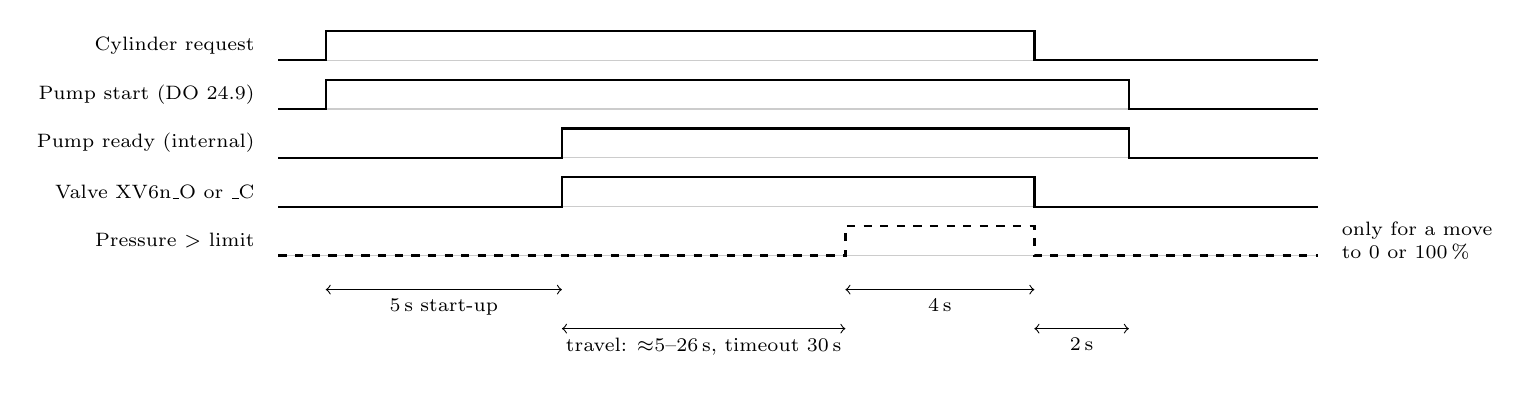
\begin{tikzpicture}[x=0.6cm, y=0.62cm, font=\scriptsize]
  \foreach \y/\l in {5/Cylinder request, 4/Pump start (DO 24.9), 3/Pump ready (internal), 2/Valve XV6n\_O or \_C, 1/Pressure $>$ limit} {
    \node[anchor=east] at (-0.3,\y+0.3) {\l};
    \draw[gray!40] (0,\y) -- (22,\y);
  }
  \draw[thick] (0,5) -- (1,5) -- (1,5.6) -- (16,5.6) -- (16,5) -- (22,5);
  \draw[thick] (0,4) -- (1,4) -- (1,4.6) -- (18,4.6) -- (18,4) -- (22,4);
  \draw[thick] (0,3) -- (6,3) -- (6,3.6) -- (18,3.6) -- (18,3) -- (22,3);
  \draw[thick] (0,2) -- (6,2) -- (6,2.6) -- (16,2.6) -- (16,2) -- (22,2);
  \draw[thick, dashed] (0,1) -- (12,1) -- (12,1.6) -- (16,1.6) -- (16,1) -- (22,1);
  \draw[<->] (1,0.3) -- node[below]{5\,s start-up} (6,0.3);
  \draw[<->] (6,-0.5) -- node[below]{travel: $\approx$5--26\,s, timeout 30\,s} (12,-0.5);
  \draw[<->] (12,0.3) -- node[below]{4\,s} (16,0.3);
  \draw[<->] (16,-0.5) -- node[below]{2\,s} (18,-0.5);
  \node[align=left, anchor=west] at (22.3,1.3) {only for a move\\to 0 or 100\,\%};
\end{tikzpicture}\end{adjustbox}
\caption{Timing of a move. For a move to an intermediate position the valve drops when the position
reaches the setpoint, without the pressure step.}
\label{fig:seq}
\end{figure}

\subsection{Pump control}
\begin{itemize}[nosep]
  \item \textbf{Auto} (default): the pump runs while any cylinder requests oil, plus 2\,s.
  \item \textbf{Manual}: the operator starts and stops the pump from the HMI
        (\var{HydraulicPump.Command.Start/Stop}).
  \item The start output is blocked by emergency stop and by starter fault
        (\var{Status.Available} = NOT \var{StarterFault}).
  \item \var{Status.Running} is the commanded state; there is no running feedback in the PLC
        \open{7}.
  \item The local panel at the HPU can also start and stop the motor [JB]. How local and remote
        start are combined is not defined \open{16}.
\end{itemize}

\subsection{Cylinder state machine}
Figure~\ref{fig:state} shows the states of one cylinder as implemented in the method
\var{CylinderStateMachine} of \var{OutletControl} (enum \var{ValveState}). The direction outputs follow the
state: \texttt{Opening} requests the open valve, \texttt{Closing} the close valve; all other states
request nothing, except jog in manual. ``Blocked'' means the cylinder has a timeout fault or no valid
position.

\begin{figure}[htbp]
\centering
\begin{adjustbox}{max width=\linewidth}\begin{tikzpicture}[font=\small, >=Stealth]
  \tikzset{st/.style={state, minimum width=24mm}, tn/.style={font=\scriptsize\bfseries, fill=white, inner sep=1pt}}
  \node[st] (cl) at (-8,0) {\textbf{Closed}\\{\scriptsize end pos.\ by pressure}};
  \node[st] (cing) at (-4,0) {\textbf{Closing}\\{\scriptsize close valve on}};
  \node[st] (ip) at (0,0) {\textbf{InPosition}\\{\scriptsize in band, valves off}};
  \node[st] (oing) at (4,0) {\textbf{Opening}\\{\scriptsize open valve on}};
  \node[st] (op) at (8,0) {\textbf{Opened}\\{\scriptsize end pos.\ by pressure}};
  \node[st, fill=red!10] (f) at (0,-3.0) {\textbf{Faulted}\\{\scriptsize valves off (KeepState)}};
  \draw[->] ([yshift=2mm]ip.west) -- node[tn, above=1pt]{T1} ([yshift=2mm]cing.east);
  \draw[->] ([yshift=-2mm]cing.east) -- node[tn, below=1pt]{T2} ([yshift=-2mm]ip.west);
  \draw[->] ([yshift=2mm]ip.east) -- node[tn, above=1pt]{T3} ([yshift=2mm]oing.west);
  \draw[->] ([yshift=-2mm]oing.west) -- node[tn, below=1pt]{T4} ([yshift=-2mm]ip.east);
  \draw[->] (cing) -- node[tn, above=1pt]{T5} (cl);
  \draw[->] (oing) -- node[tn, above=1pt]{T6} (op);
  \draw[->] (op.north) -- ++(0,0.9) -| node[tn, pos=0.25, above=1pt]{T7} (cing.north);
  \draw[->] (cl.south) -- ++(0,-1.1) -| node[tn, pos=0.25, below=1pt]{T8} (oing.south);
  \draw[->, red!70!black] ([xshift=-4mm]ip.south) -- node[tn, left=1pt, pos=0.75]{T9} ([xshift=-4mm]f.north);
  \draw[->] ([xshift=4mm]f.north) -- node[tn, right=1pt, pos=0.25]{T10} ([xshift=4mm]ip.south);
\end{tikzpicture}\end{adjustbox}

\vspace{2mm}
\begin{small}
\begin{tabularx}{\linewidth}{@{}lL@{}}
\toprule
T & Condition (hyst.\ = \var{PositionCounterHysteresis}, SP = ramped setpoint) \\
\midrule
T1 & pos $>$ SP + hyst., or SP = 0 and pos $>$ 0 (a move to 0\,\% always ends on pressure) \\
T2 & pos $\le$ SP and SP $>$ 0 \\
T3 & pos $<$ SP $-$ hyst., or SP = 100 and pos $<$ 100 \\
T4 & pos $\ge$ SP and SP $<$ 100 \\
T5 / T6 & End position confirmed: driven-side pressure $>$ limit for 4\,s \\
T7 & pos $>$ SP + hyst.\ and SP $<$ 100 \\
T8 & pos $<$ SP $-$ hyst.\ and SP $>$ 0 \\
T9 & Blocked: timeout fault, or no valid position. Applies to every state, drawn for InPosition only \\
T10 & Not blocked any more; InPosition then picks the direction \\
\bottomrule
\end{tabularx}
\end{small}
\caption{State diagram of one cylinder (\texttt{ValveState}; the transient \texttt{MovingToPosition}
goes straight to \texttt{InPosition}). Emergency stop does not change the state; it switches both
valves off and freezes the ramped setpoint at the actual position.}
\label{fig:state}
\end{figure}

\paragraph{Fault action.} The PLC calls the state machine with \var{FaultActionMode.KeepState}: in
\texttt{Faulted} both valves are off and the cylinder stays where it is. The modes \texttt{Close}
and \texttt{Open} exist in the code but are not used. This matches the power-loss decision
\decided{1}: the outlet is never moved automatically to a safe end position.

\paragraph{Fault recovery.} The timeout fault is the alarm state of the travel-time alarm. When the
valve drops, the timer resets; when the operator acknowledges, the alarm returns to normal and the
cylinder leaves \texttt{Faulted}. From \texttt{InPosition} it will try again if the position is
still outside the band. \var{Command.FaultReset} exists in the DUT but is not used.

% =====================================================================================================
\section{Functional requirements}
\label{sec:freq}
Requirements are numbered FR-n. ``Impl.'' marks requirements the current PLC export meets.

\subsection{Processes}
\begin{description}[nosep, leftmargin=14mm, style=sameline]
  \item[FR-1] The system shall hold all four dampers at the opening of the selected operating mode
        (auto). \hfill Impl.
  \item[FR-2] The operator shall be able to set a common manual opening, and to put each cylinder
        in manual with its own setpoint and jog. \hfill Impl.
  \item[FR-3] The position of each cylinder shall be computed from flow meter pulses, 0--100\,\%.
        \hfill Impl.
  \item[FR-4] Moves to 0 and 100\,\% shall end on a pressure-confirmed end position. \hfill Impl.
        for the side with a transmitter \open{1}
  \item[FR-5] The pump shall run only while a cylinder needs oil (auto), or on operator command
        (manual). \hfill Impl.
  \item[FR-6] The operator shall be able to calibrate closed and open positions per cylinder, and
        the PLC shall check the calibration at every end position. \hfill Impl.
\end{description}

\subsection{Inputs and outputs}
The inputs are the four pulse counters, the pressure transmitters, the tank switch, the starter
fault and the emergency stop; the outputs are eight solenoid valves and the pump start. The full
list with addresses is Table~\ref{tab:io}; ranges and resolution are in Table~\ref{tab:instr}.
\begin{description}[nosep, leftmargin=14mm, style=sameline]
  \item[FR-7] All JB1 signals that the operator needs to act on shall be wired to the PLC:
        filter clogged, motor running, motor overload, E-stop pressed, power supply state
        \open{6}\open{7}.
  \item[FR-8] The pressure transmitters shall be scaled 0--250\,bar in the retained configuration.
        The DUT default is 0--10; the simulator \var{ConfigValues} set 0--250 \open{4}.
\end{description}

\subsection{Start-up and shut-down}
\begin{description}[nosep, leftmargin=14mm, style=sameline]
  \item[FR-9] After a PLC restart the mode, the mode table, the calibration (closed/open counts),
        the last counter value and the transmitter configuration shall be restored from retain
        memory. \hfill Impl.
  \item[FR-10] After a restart or a loss of the remote I/O link, no cylinder shall move until the
        link has been up for 1\,s and the counter values are valid. If a counter module has
        restarted at 0, the retained count shall be written back first. \hfill Impl.
  \item[FR-11] A restart shall not move the dampers by itself, except to bring a cylinder that
        is outside the hysteresis band back to its setpoint. \hfill Impl.
  \item[FR-12] First commissioning: each cylinder shall be calibrated (close fully, define closed;
        open fully, define open) before auto is used. The default span of 2000 pulses is treated as
        calibrated by the PLC, so this relies on the commissioning procedure \open{15}.
  \item[FR-13] Shut-down: on emergency stop the pump stops and all valves drop. The dampers stay
        where they are. \hfill Impl.
\end{description}

\subsection{Power loss}
\label{sec:power}
\textbf{Decision \decided{1} (21.10.2026):} the outlet does \emph{not} close automatically on
power loss.
\begin{itemize}[nosep]
  \item The dampers hold their position: the over-centre valves lock the cylinders, and the PLC
        fault action is \var{KeepState}.
  \item If the outlet must be moved without power, the operator does it by hand at the HPU: the hand
        pump (\itag{HP61}\prop) gives pressure, and the valve section is shifted by its manual
        actuator \open{17}.
  \item An accumulator for automatic closing is deferred. The HPU cabinet has room to retrofit
        one later if needed.
  \item JB1 has a backup 400\,V supply (K2) for the pump; how it is selected is open \open{6}.
\end{itemize}
This supersedes [FD] rev.~B §3.2.3 ``Utløpet skal stenge ved strømbortfall'' (fail to close) and the
shut-off valve \itag{XV65}. XV65 is not on [A1]; its DO (24.8) and cable are spare.

\begin{description}[nosep, leftmargin=14mm, style=sameline]
  \item[FR-14] A ``power lost / pump on backup supply'' signal from the HPU (relay contact, [AKS]
        item 82) shall reach the PLC, and the operator shall get an alarm \open{6}.
\end{description}

\subsection{Fault identification and recovery}
Table~\ref{tab:alarms} lists the alarms. Common rules:
\begin{description}[nosep, leftmargin=14mm, style=sameline]
  \item[FR-15] A cylinder whose valve is on for longer than the travel time shall stop and give an
        alarm (\emph{long opening / closing time}). It stays stopped until the alarm is
        acknowledged. \hfill Impl.
  \item[FR-16] Count changes without an active valve, a wrong count direction, or a counter set that
        is not confirmed shall give a \emph{position measurement fault}. \hfill Impl.
  \item[FR-17] A deviation between counted and pressure-confirmed end position larger than the
        tolerance shall give a \emph{calibration} warning. \hfill Impl.
  \item[FR-18] Low oil level or high oil temperature shall give an alarm. Whether it shall also
        stop the pump is open \open{9}.
  \item[FR-19] Emergency stop, clogged filter and motor overload shall each give an alarm
        \open{7}\open{8}.
\end{description}

\subsection{Communication}
\begin{description}[nosep, leftmargin=14mm, style=sameline]
  \item[FR-20] The PLC reads and writes the CommonRIO image over Modbus TCP every cycle. A lost link
        gives the alarm \emph{CommonRIO communication error}; the cylinder positions become invalid
        and the cylinders go to \texttt{Faulted} (valves off). \hfill Impl.
  \item[FR-21] On a lost link the remote I/O shall switch its outputs (valves, pump start) off, so
        the dampers hold. The behaviour of the 750-362 fieldbus watchdog is not set, and [FD]
        Tabell~4 is empty \open{13}.
  \item[FR-22] The HMI shall show per cylinder: position, setpoint, state, valve outputs, line
        pressure, calibration status and alarms; and for the HPU: pump state, tank and filter
        status, power supply state.
\end{description}

% =====================================================================================================
\section{Non-functional requirements}
\label{sec:nfreq}

\subsection{Timing and capacity}
\label{sec:timing}
Table~\ref{tab:calc} gives estimates from the cylinder data and the pump flow. [FD] leaves the
stroke time open (``ca nn sekunder''); these numbers should replace it after the FAT.

\begin{table}[htbp]
\centering
\caption{Estimated stroke times, pulse counts and pulse rates.}
\label{tab:calc}
\begin{small}
\begin{tabularx}{\textwidth}{@{}LP{50mm}r@{}}
\toprule
Quantity & Basis & Value \\
\midrule
Oil volume, plus stroke (A side) & $\pi\cdot 2.0^2\,\text{cm}^2 \cdot 30\,\text{cm}$ & 0.377\,l \\
Oil volume, minus stroke (B side) & $\pi(2.0^2-1.0^2)\,\text{cm}^2 \cdot 30\,\text{cm}$ & 0.283\,l \\
Pulses per full stroke (A line, both directions) & $377\,\text{cm}^3 / 0.191\,\text{cm}^3$ & $\approx$1970 \\
\quad [FD] / PLC default span & 0.4\,l $\times$ 5200 / default \var{OpenPosition} & 2080 / 2000 \\
Position resolution & 1 pulse & 0.05\,\% $\approx$ 0.15\,mm \\
Stroke time, one cylinder alone, plus / minus & 0.377\,l and 0.283\,l at 3.5\,l/min & 6.5\,s / 4.9\,s \\
Stroke time, four cylinders together, plus / minus & 1.51\,l and 1.13\,l at 3.5\,l/min & 26\,s / 19\,s \\
\quad add pump start-up & \var{PumpStartUpTime} & 5\,s \\
Travel timeout & \var{MaxTravelTimeOpen/Close} & 30\,s \\
Pulse rate, all four moving & $\approx$0.9\,l/min per cylinder & $\approx$75\,Hz \\
Pulse rate, one cylinder, plus stroke & 3.5\,l/min (4.1\,l/min unloaded) & 300\,Hz (355\,Hz) \\
Pulse rate, one cylinder, minus stroke & A-side outflow = pump flow $\times$ 12.57/9.42 = 4.7 (5.4)\,l/min & 410\,Hz (470\,Hz) \\
750-638 max.\ input frequency & data sheet & 500\,Hz \\
QG100 measuring range & data sheet & 0.05--5\,l/min \\
\bottomrule
\end{tabularx}
\end{small}
\end{table}

Findings:
\begin{itemize}[nosep]
  \item A full plus stroke of all four cylinders takes about 26\,s of valve-on time. The travel
        timeout of 30\,s leaves about 4\,s (15\,\%). Cold oil, wear and the over-centre back pressure
        can use that up, and the move then ends in a fault. The timeout should be set from FAT
        measurements, e.g.\ 1.5$\times$ the measured time \open{4}.
  \item The design basis and simulator assume 30\,s per stroke and a 160\,bar relief [DB]; they
        should be updated to the numbers above and to [A1] \open{3}.
  \item A single cylinder on the minus stroke pushes about 4.7--5.4\,l/min out through its flow
        meter: at or above the top of the QG100 range and close to the 500\,Hz of the 750-638. Jog
        of one cylinder on the minus stroke is the worst case. Check the count at the FAT \open{11}.
  \item The QG100 is calibrated in the arrow direction; accuracy in reverse flow (minus stroke) is
        not stated \open{11}. The end-position check catches a drift, but only at end positions.
\end{itemize}

Other timing: PLC cycle and Modbus TCP update are fast compared with the pulse period at the
setpoint (300\,Hz $\to$ 3\,ms per pulse; 5\,\% hysteresis = $\approx$100 pulses), so the overshoot
after the valve drops is small compared with the hysteresis. Pressure end-position delay 4\,s;
direction check delay 2\,s; counter-set timeout 3\,s; comm valid delay 1\,s.

\subsection{Pressure thresholds}
\begin{small}
\begin{tabularx}{\textwidth}{@{}LrP{60mm}@{}}
\toprule
Setting & Value & Source / comment \\
\midrule
Main relief valve & 150\,bar & [A1]; design 170, test 190\,bar \\
Over-centre valves, A and B & 130\,bar & [A1] ([T1]: 110\,bar) \\
Port pressure limiters & 100\,bar & [A1] \\
PLC end-position limit \var{MaxPressureOpen/Close} & 100\,bar & \var{CylinderConfigDUT} default; must be below the port limiter, e.g.\ 70--80\,bar, and above the running pressure (\TBD, measure at FAT) \open{3} \\
End-position delay & 4\,s & \var{MaxPressureOpen/CloseDelay} \\
Transmitter range & 0--250\,bar & PT5401; PLC scaling must match \open{4} \\
\bottomrule
\end{tabularx}
\end{small}

\subsection{Alarms}
\begin{table}[htbp]
\centering
\caption{Outlet alarms. Status: Impl.\ = in the PLC export; FD = in [FD]/[AL] but not in the PLC; Prop.\ = proposed here.}
\label{tab:alarms}
\begin{small}
\begin{tabularx}{\textwidth}{@{}P{34mm}LP{26mm}P{26mm}P{12mm}@{}}
\toprule
Alarm & Condition & Delay / limit & Action & Status \\
\midrule
Long opening time, cyl.\ n & Open valve on longer than limit & 30\,s (travel time open) & Valve off, cylinder faulted until ack. & Impl. \\
Long closing time, cyl.\ n & Close valve on longer than limit & 30\,s (travel time close) & As above & Impl. \\
Position measurement fault, cyl.\ n (\var{FlowSensorFault}) & Drift $>$ 2 pulses without valve; or counting direction wrong; or counter set not confirmed & 0.5\,s / 2\,s / 3\,s & Alarm; position invalid while direction wrong & Impl. \\
Calibration error, cyl.\ n & $|$counted $-$ end position$|$ $>$ tolerance at a confirmed end, or position outside $-5\ldots105$\,\% & 5\,\% (calibration tolerance) & Warning; recalibrate & Impl. \\
Pressure transmitter fault, cyl.\ n & Wire break / out of range (AnalogSensor) & module status & Alarm & Impl. \\
Low level / high temperature, hydraulic tank & LSL61 or TSH61 (series) & none in PLC; [FD]: configurable & Alarm only \open{9} & Impl. \\
Hydraulic pump starter fault & DI 44.0 (motor overload QM1) & -- & Pump not available & Impl. \\
CommonRIO communication error & Modbus TCP link down & -- & Positions invalid, valves off & Impl. \\
Emergency stop activated & ES61 & -- & Pump and valves off (done); alarm missing & FD \open{8} \\
Filter clogged & PDS61/PDS62 & \TBD & Alarm, change filter & Prop.\ \open{7} \\
Power lost / pump on backup & relay from HPU & \TBD & Alarm & Prop.\ \open{6} \\
Motor not running & start on, no running feedback & \TBD & Alarm & Prop.\ \open{7} \\
\bottomrule
\end{tabularx}
\end{small}
\end{table}
The flow deviation alarms of [FD] Tabell~11 (estimated inflow too low / too high) belong to the
inlet and level function and are not repeated here.

\subsection{Parameters}
All parameters below are retained in \var{GVLRetain} (outlet configuration, cylinder
configuration, transmitter configuration and last counter value per cylinder) and can be changed on
the HMI. The values are the DUT defaults; production values are \TBD{} until the FAT.
\begin{small}
\begin{longtable}{@{}P{48mm}P{22mm}P{80mm}@{}}
\caption{Outlet parameters (\texttt{OutletConfigDUT}, \texttt{CylinderConfigDUT}) and fixed constants.}\label{tab:param}\\
\toprule
Parameter & Default & Meaning \\
\midrule
\endfirsthead
\toprule
Parameter & Default & Meaning \\
\midrule
\endhead
\bottomrule
\endfoot
\var{ModePosition[O35..S75]} & 20, 30, 40, 50\,\% & Opening per mode \open{5} \\
\var{Mode} & O35 & Selected mode (retained) \\
\var{MaxPressureOpenDelay} / \var{CloseDelay} & 4\,s & Pressure above limit this long = end position \\
\var{MaxTravelTimeOpen} / \var{Close} & 30\,s & Travel timeout; also jog limit (0 = no jog limit) \open{4} \\
\var{RampRateOpen} / \var{Close} & 0\,\%/s & Setpoint ramp, 0 = off \\
\var{PositionCounterHysteresis} & 5\,\% & Dead band around the setpoint \\
\var{CalibrationTolerance} & 5\,\% & Calibration check at end positions (min.\ 0.5\,\%) \\
\var{PumpStartUpTime} & 5\,s & Pump runs this long before valves open ([FD]: 5\,s) \\
\var{PumpStopDelay} & 2\,s & Pump keeps running after the last request \\
\var{EnableTimeoutAlarms} & TRUE & FALSE suppresses the travel timeout alarms \emph{and} the fault \\
\midrule
\var{ClosedPosition} (per cyl.) & 0 & Counter value at closed \\
\var{OpenPosition} (per cyl.) & 2000 & Counter value at open (calibrated $\approx$1970) \\
\var{MaxPressureOpen} / \var{Close} (per cyl.) & 100\,bar & End-position pressure limit \open{3} \\
\var{PressureOpen/Close.Config} (per cyl.) & 0--10 (DUT); 0--250 (sim) & Transmitter scaling \open{4} \\
\midrule
\var{DIRECTION_DELAY} & 2\,s & Constant: direction mismatch tolerated \\
\var{DRIFT_LIMIT} & 2 pulses & Constant: drift without valve ([FD], HOLD) \open{18} \\
\var{ZERO_BAND} / \var{JUMP_LIMIT} & 5 / 50 pulses & Constant: counter restart detection \\
\var{COUNTER_SET_TIMEOUT} & 3\,s & Constant: set-counter handshake \\
Fault action & KeepState & Constant in the call; matches \decided{1} \\
\end{longtable}
\end{small}

\subsection{Instruments}
% casfd's instrument table columns are 160 mm plus column separation; narrow the separation to fit the text width
{\setlength{\tabcolsep}{1.3pt}
\begin{instrumenttable}{Outlet instruments and actuators (typical cylinder n = 1..4; tags per [PID]).}\label{tab:instr}
\itag{FT61}..\newline\itag{FT64} & Oil flow to/from A side, position by pulse count & HPU cabinet, A line & Pulse 24\,V, 3-wire, to 750-638 & 0.05--5\,l/min & 0.191\,cm$^3$ (0.05\,\%) & Control \\
\itag{PT61}, \itag{PT63},\newline \itag{PT65}, \itag{PT67} & Pressure A side (plus stroke), end position & HPU cabinet, A line & 4--20\,mA to 750-455 & 0--250\,bar & $\approx$0.12\,bar & Control, alarm \\
\itag{PT62}, \itag{PT64},\newline \itag{PT66}, \itag{PT68} & Pressure B side (minus stroke) & -- & 4--20\,mA, AI reserved & 0--250\,bar & -- & Not installed \open{1} \\
\itag{XV61}..\newline\itag{XV64} & Directional valve, \_O / \_C solenoids (MB1--MB8) & HPU valve bank & DO 750-1515 via relays XK, 24\,V 680\,mA & on / off & -- & Control \\
\itag{PU61}/\newline\itag{M61} & Hydraulic pump and motor & HPU & DO start (KM1), DI overload & 3.5\,l/min, 150\,bar & -- & Control \\
\itag{LSL61}/\newline\itag{TSH61} & Tank low level / oil temperature high & HPU tank & DI, NC, series & 120\,mm / 70\,$^\circ$C & -- & Alarm \\
\itag{PDS61}\prop/\newline\itag{PDS62}\prop & Pressure / return filter clogged & HPU & DI, series & 5 / 1.5\,bar $\Delta p$ & -- & Alarm (prop.) \\
\itag{ES61} & Emergency stop & Panel ST-16183 & DI, NC loop & -- & -- & Interlock \\
\itag{PI61} & Pressure gauge & HPU & local & 0--250\,bar & -- & Local \\
\itag{ZI61}..\newline\itag{ZI64} & Damper position (computed) & PLC & -- & 0--100\,\% & 0.05\,\% & HMI \\
\end{instrumenttable}}

\subsection{I/O list}
\begin{small}
\begin{longtable}{@{}P{30mm}P{26mm}P{22mm}P{68mm}@{}}
\caption{Outlet I/O on CommonRIO (Modbus TCP image, [PLC] \texttt{FB.RIO.CommonRIO}; modules per [PID]).}\label{tab:io}\\
\toprule
Module / ch. & Image & JB1 terminal & PLC variable \\
\midrule
\endfirsthead
\toprule
Module / ch. & Image & JB1 terminal & PLC variable \\
\midrule
\endhead
\bottomrule
\endfoot
\multicolumn{4}{@{}l}{\textit{Inputs}}\\
-R1-004 750-638 ch1/2 & IN 12/13, 14/15 & X2:1--6 & \var{Outlet.Cylinder[0..1].Input.OilFlowStatusWord} / \var{OilFlowCounter} \\
-R1-005 750-638 ch1/2 & IN 16/17, 18/19 & X2:7--12 & \var{Outlet.Cylinder[2..3].Input...} \\
-R1-009 750-455 ch1--4 & IN 28--31 & X1:3--7 & \var{Cylinder[0].PressureOpen} (28), \var{Cylinder[0].PressureClose} (29, no PT), \var{Cylinder[1]} (30, 31) \\
-R1-010 750-455 ch1--4 & IN 32--35 & X1:8--12 & \var{Cylinder[2]} (32, 33), \var{Cylinder[3]} (34, 35); odd words have no PT \open{1} \\
-R1-017 750-1405 ch1 & IN 44.0 & X1:25 & \var{HydraulicPump.Input.StarterFault} \\
-R1-017 750-1405 ch2 & IN 44.1 & X1:1--2 & \var{Outlet.Input.HydraulicOilTankFault} \\
-R1-017 750-1405 ch3 & IN 44.2 & X1:26--35 & \var{GVLMain.EmergencyStop} := NOT 44.2 (NC loop) \\
-R1-017 750-1405 ch4.. & IN 44.3.. & X1:13--24, 26--35 & Spare: filter, motor running, local start/stop, power state \open{6}\open{7} \\
\multicolumn{4}{@{}l}{\textit{Outputs}}\\
-R1-004/005 750-638 & OUT 12--19 & -- & \var{OilFlowControlWord} / \var{OilFlowCounterSet} per cylinder \\
-R1-019 750-1515 ch1--8 & OUT 24.0--24.7 & X2:13--24 & \var{Cylinder[0..3].Output.OpenValve} / \var{CloseValve}, via relays XK01--XK08 \\
-R1-020 750-1515 ch1 & OUT 24.8 & -- & Spare (was XV65, superseded \decided{1}) \\
-R1-020 750-1515 ch2 & OUT 24.9 & X1:23 & \var{HydraulicPump.Output.Start} \\
-R1-020 750-1515 ch3 & OUT 24.10 & -- & \var{HydraulicPump.Output.Reset}: no counterpart \open{7} \\
-R1-020 750-1515 ch4.. & OUT 24.11.. & X1:21--22 & Spare: activate main / backup supply \open{6} \\
\end{longtable}
\end{small}
Cabinet drawing 792.001 rev.~1 still shows DI module -R1-017 and DO -R1-020 ch2/3 as spare; they
must be wired for the PLC mapping above [PID]. The header comment in \var{CommonRIO.OutputMapping}
names the DO modules -R1-018/019 and ``750-455''; the P\&ID set has -R1-019/020 750-1515.

\subsection{HMI operator functions}
The HMI screens for the outlet are not built yet \open{19}. The PLC offers these commands:

\begin{small}
\begin{tabularx}{\textwidth}{@{}P{48mm}L@{}}
\toprule
Function & PLC interface \\
\midrule
Select operating mode & \var{Outlet.Command.Mode} (O35..S75; invalid values ignored) \\
Edit mode openings & \var{Outlet.Config.ModePosition[]} \\
Outlet auto / manual, manual position & \var{Outlet.Command.Auto/Manual}, \var{ManualPosition} \\
Cylinder auto / manual, setpoint & \var{Outlet.Cylinder[i].Command.Auto/Manual}, \var{ManualSetpoint} \\
Jog open / close (hold to run) & \var{Outlet.Cylinder[i].Command.Open/Close} \\
Define closed / open position & \var{Outlet.Cylinder[i].Command.CalibrateClosed/CalibrateOpen} \\
Pump auto / manual, start / stop & \var{Outlet.HydraulicPump.Command.Auto/Manual/Start/Stop} \\
Acknowledge alarms & \var{Outlet.Cylinder[i].AlarmAck.*}, \var{Outlet.AlarmAck.*}, \var{HydraulicPump.AlarmAck.*} \\
Show & position, setpoint, target, state, valve outputs, pressures, calibration deviation, pump state \\
\bottomrule
\end{tabularx}
\end{small}

Some outlet commands exist in the DUT but are not used by the code: \var{Open}, \var{Close},
\var{FaultReset}, \var{ManualPumpStart} and \var{ManualPumpStop}.

\subsection{Verification}
The outlet simulator CasOutletSim (heimdall-cas-simulation) models piston, pulses and line
pressures, and injects jammed cylinder, counter drift, transmitter faults and a pump that runs
without pressure [DB]. The integrated FAT with the Servi cabinet at Østerbø is planned for the end of
October 2026. It should at least measure: stroke times (single and four together, both directions),
running and end-stop pressures, pulses per full stroke both ways, drift with the valves in neutral,
the minus-stroke pulse rate, the valve response to on/off relay drive, and the emergency-stop and
power-loss behaviour \open{20}.

% =====================================================================================================
\section{Open issues and decisions}
\label{sec:open}

\subsection{Decisions}
\begin{small}
\begin{tabularx}{\textwidth}{@{}lP{20mm}L@{}}
\toprule
No. & Date & Decision \\
\midrule
DEC1 & 21.10.2026 & The outlet does not close automatically on power loss. Dampers hold position (over-centre valves, PLC
  \var{FaultActionMode.KeepState}); manual override with the hand pump at the HPU. Accumulator deferred; there is space in the
  cabinet to retrofit it. Supersedes [FD] rev.~B fail-to-close and XV65. \\
DEC2 & 16.10.2026 & One multi-core signal cable with common 24\,V / 0\,V, bridged in JB1; separate conductors for the valve
  coils [MAIL]. \\
\bottomrule
\end{tabularx}
\end{small}

\subsection{Open issues}
\begin{small}
\begin{longtable}{@{}lP{100mm}P{30mm}@{}}
\toprule
No. & Issue & Owner / next step \\
\midrule
\endfirsthead
\toprule
No. & Issue & Owner / next step \\
\midrule
\endhead
\bottomrule
\endfoot
OI1 & \textbf{One pressure transmitter per cylinder.} [A1] has 1PT1--1PT4 on the A line only; [FD] (PT61--68),
  the P\&ID and the PLC (8 AIs, \var{PressureOpen} + \var{PressureClose}) expect two. The minus-stroke end cannot be confirmed;
  with \var{MaxPressureClose} $>$ 0 a move to 0\,\% ends in a travel timeout. Options: buy a second transmitter on a Minimess
  point (Servi offered, 19.10, extra cost), or detect end of stroke by pulses stopping (PLC change). Bjørn asked 19.10 who
  removed 4 of 8. & JP / Bjørn / Servi \\
OI2 & \textbf{Plus stroke = open?} PLC and P\&ID assume A side / plus stroke opens the damper. Confirm with Østerbø's damper
  linkage; it decides which end the single PT confirms and whether \var{CalibrateOpen} is possible. & Østerbø \\
OI3 & \textbf{End-position limit vs port limiter.} PLC limit 100\,bar (strict $>$) equals the 100\,bar port limiters of [A1];
  may never trip. Set below (e.g.\ 70--80\,bar) after measuring running pressure. Also align [DB]/simulator (160\,bar relief,
  40\,bar load assumed). & Bjørn / FAT \\
OI4 & \textbf{Travel timeout and scaling.} Four cylinders together need $\approx$26\,s; \var{MaxTravelTime} 30\,s has little margin.
  [FD] ``ca nn s'' to be filled in. PT scaling DUT default 0--10; production retain must be 0--250\,bar. & Bjørn / FAT \\
OI5 & \textbf{Mode openings.} [FD] column empty; PLC default [20, 30, 40, 50]\,\% rises while flow falls (looks reversed). Need
  openings per mode and the stroke $\to$ opening relation. & Østerbø / process \\
OI6 & \textbf{Power state to the PLC.} ``Power lost / pump on backup'' relay ([AKS] 82) not on [JB]; K1/K2 ``activate main / backup''
  inputs on [JB] are not mapped. Who selects the backup supply (PLC, PMS, local)? Alarm wanted. & JP / Servi / Bjørn \\
OI7 & \textbf{JB1 signals not mapped.} Filter clogged, motor running, motor overload (assumed = \var{StarterFault}), E-stop
  pressed / loop. PLC \var{Reset} output (24.10) has no counterpart (QM1 manual). Wire DI -R1-017 and DO -R1-020. & Bjørn / Knut \\
OI8 & \textbf{Missing alarms.} No emergency-stop alarm (ES61 in [AL]); no filter, overload, motor-not-running or power alarms. & Bjørn \\
OI9 & \textbf{Oil tank fault only alarms.} Low level / 70\,$^\circ$C does not stop the pump; no delay as [FD] asks. Decide
  whether to stop the pump (pump protection). & Bjørn / Servi \\
OI10 & \textbf{Flow meter signal.} [JB] overview sheet says 4--20\,mA, rev.~A2 says pulse (PLC assumes pulse); Servi to correct
  the overview. The direction output of the QG100 (type 46) is unused. & Servi \\
OI11 & \textbf{Pulse rate and reverse flow.} One cylinder on the minus stroke: 4.7--5.4\,l/min, 410--470\,Hz, at the top of the
  QG100 range and near the 500\,Hz 750-638 limit. Reverse-flow accuracy of the QG100 not stated. Test at FAT. & FAT \\
OI12 & \textbf{PSL valves on/off.} The PSL sections are proportional; [JB] sheet 8 shows an amplifier option ($\pm$10\,V, 0.63\,A,
  4--20\,mA setpoint). The PLC drives the 24\,V coils (680\,mA) on/off through relays XK. Confirm with Servi that full on/off
  drive is right (min.\ $\approx$250\,mA [QNA], optional speed card) and the relay contact rating. & Servi / Knut \\
OI13 & \textbf{Comm-loss output behaviour.} [FD] Tabell~4 empty; 750-362 watchdog not configured. Proposed: valves and pump start off (hold). & Bjørn \\
OI14 & \textbf{Data disagree.} Motor 1.5\,kW 400\,V ([A1], [TDS], [JB]) vs ``under 1\,kW'' ([QNA]); [JB] cable -W1M1 labelled ``24Vdc'';
  pressures 150/130\,bar ([A1]) vs 160/110 ([DB], [T1]); tank 12\,l ([A1]) vs 10\,l in earlier notes; cylinder type
  also written ``HCR-C-D-40/20x300'' vs ``HRC-N-D-40/20x300'' on the [A1] part list. Motor starter location [AKS] 91. & JP / Servi \\
OI15 & \textbf{Calibration state.} The default span (0--2000) counts as calibrated; no ``never calibrated'' state. Calibration
  must be part of commissioning. \var{Command.FaultReset} unused. & Bjørn \\
OI16 & \textbf{Local / remote.} Local Start / Stop on ST-16183 is not in the PLC; priority between local panel and PLC start, and
  whether E-stop also removes coil power, not defined. & Servi / Bjørn \\
OI17 & \textbf{Manual override and exercise.} Write the hand-pump procedure (which valve to operate, manual levers on the PSL
  sections to be confirmed) and the weekly end-position exercise into the O\&M manual. & Østerbø / Servi \\
OI18 & \textbf{Drift limit.} 2 pulses (HOLD in [FD]); check against measured leakage and thermal drift with the over-centre valves. & FAT \\
OI19 & \textbf{HMI.} Outlet screens not built; content per this document. & HMI \\
OI20 & \textbf{Integrated FAT} at Østerbø (end of October 2026): test plan per the verification section. & Fredrik / JP \\
\end{longtable}
\end{small}

\end{document}
